\documentclass[color,refNum]{ECEHW}

\usepackage{sourcehan}
\usepackage{metalogo}

\ECEHWsetup{
  title        = {\boldSong 中文测试},
  version      = {$1^{\mathrm{st}}$},
  author       = {金宇琛},
  subject      = {ECE ????},
  organization = {University of Houston},
  codeStyle    = {default}
}

\mdtheorem[style=exercisestyle]{cexercise}{\textbf{练习}}
\providecommand*{\cexerciseautorefname}{练习}
\mdtheorem[style=theoremstyle]{ctheorem}{\textbf{定理}}
\providecommand*{\ctheoremautorefname}{定理}

%===========================================================
\begin{document}
	
\maketitle

本字体包需要用户在自己的电脑上安装思源宋体和思源黑体,这两个字体是开源的,用户可以到以下两个链接下载:

\begin{enumerate}
  \item 思源宋体:\url{https://source.typekit.com/source-han-serif/}
  \item \textsf{思源黑体}:\url{https://github.com/adobe-fonts/source-han-sans/tree/release}
\end{enumerate}

需要注意的是,本宏包只是为{\XeLaTeX}设计的,虽然它也能支持{pdf\LaTeX}和{\LuaLaTeX},但是后两者的效果会fallback到没有思源宋体和思源黑体的状态。

\section{基本中文范例}

首先,我们展示一些中文范例:

\begin{table}[htbp]
  \vspace{-1.5em}
  \centering
  \caption{思源宋体范例列表 \label{tab:song}}
  \begin{tabular}{|c|m{0.38\textwidth}|}
    \hline
    字重 & \makebox[0.38\textwidth][c]{范例} \\ \hline
    普通 & 小楼昨夜又东风,故国不堪回首月明中。 \\ \hline
    \multirow{2}{*}{半粗} & \textbf{小楼昨夜又东风,故国不堪回首月明中。} \\ \cline{2-2}
     & {\semiSong 小楼昨夜又东风,故国不堪回首月明中。} \\ \hline
    \multirow{2}{*}{粗} & {\semiSong \textbf{小楼昨夜又东风,故国不堪回首月明中。}} \\ \cline{2-2}
    & {\boldSong 小楼昨夜又东风,故国不堪回首月明中。} \\ \hline
    极粗 & {\boldSong \textbf{小楼昨夜又东风,故国不堪回首月明中。}} \\ \hline
  \end{tabular}
\end{table}

并展示一些黑体中文范例。黑体由\texttt{$\backslash$textsf}提供:

\begin{table}[htbp]
  \vspace{-1.5em}
  \centering
  \caption{思源宋体范例列表 \label{tab:hei}}
  \begin{tabular}{|c|m{0.35\textwidth}|}
    \hline
    字重 & \makebox[0.35\textwidth][c]{范例} \\ \hline
    普通 & \textsf{雕栏玉砌应犹在,只是朱颜改。} \\ \hline
    \multirow{2}{*}{半粗} & \textbf{\textsf{雕栏玉砌应犹在,只是朱颜改。。}} \\ \cline{2-2}
    & {\semiHei 雕栏玉砌应犹在,只是朱颜改。} \\ \hline
    \multirow{2}{*}{粗} & {\semiHei \textbf{雕栏玉砌应犹在,只是朱颜改。}} \\ \cline{2-2}
    & {\boldHei 雕栏玉砌应犹在,只是朱颜改。} \\ \hline
    极粗 & {\boldHei \textbf{雕栏玉砌应犹在,只是朱颜改。}} \\ \hline
  \end{tabular}
\end{table}

最后是一个楷体范例:{\kai 东风夜放花千树,更吹落,星如雨。}

和一个仿宋范例:\texttt{宝马雕车香满路,凤箫声动,玉壶光转,一夜鱼龙舞。}

\section{中文替换功能}

当启用中文支持时,包括图、表名字,摘要和参考文献标题在内的一些功能会被自动换成中文。定理环境不允许替换已经定义的定理名字,因此一种解决方案是定义一个新的使用中文命名的定理,如同以下的例子。

其他的一些更复杂的自定义环境、命令是无法简单地被替换成中文的,对于这种情况,仍然需要用户在使用中文的时候,手动修改原模板。

\begin{cexercise}[问题 2.1]
	测试子图功能,让我们引用一下\autoref{fig:ex1:resD:2},以及\autoref{thm:1}。
    
  \begin{figure}[H]
  	\centering
  	\begin{minipage}[b]{0.48\textwidth}
  		\centering
  		\subfigure[$D=1$]{
  			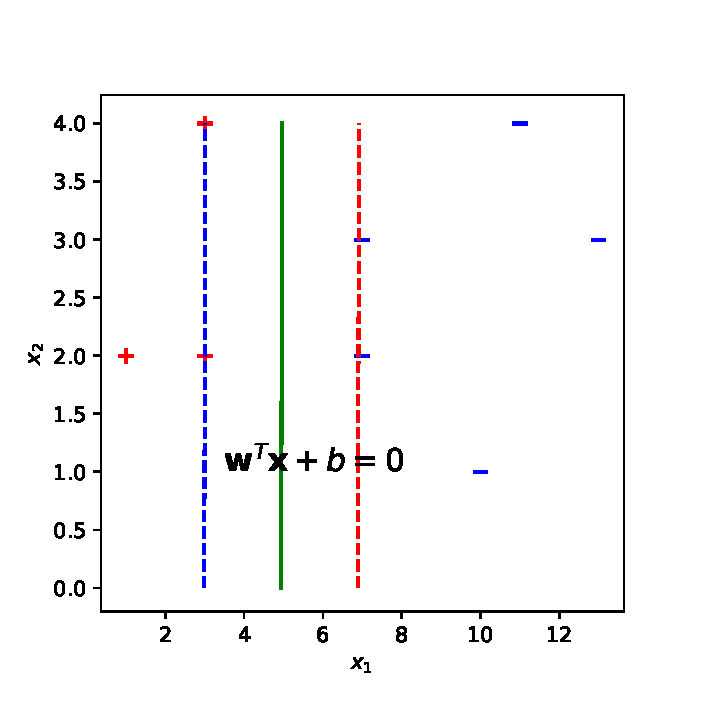
\includegraphics[width = 0.7\columnwidth]{pic-ex}
  		}
  	\end{minipage}
  	\begin{minipage}[b]{0.48\textwidth}
  		\centering
  		\subfigure[$D=0.5$]{ \label{fig:ex1:resD:2}
  			Here could be a graph.
  		}
  	\end{minipage}
  	\DeclareGraphicsExtensions.
  	\caption{Test graphs.}
  	\label{fig:ex1:resD}
  \end{figure}

  \begin{ctheorem}[放在问题里的定理] \label{thm:1}
    \vspace{0.5em}
    check the theorem.
  \end{ctheorem}

	\qED
	
\end{cexercise}

\begin{ctheorem}[一个中文定理]
  这个定理是重新手动定义的。引用了一下\cite{Dong7115171,Yang6175956}。
\end{ctheorem}

%\phantomsection
%\addcontentsline{toc}{section}{\refname}
\bibliographystyle{IEEEtran}
% argument is your BibTeX string definitions and bibliography database(s)
\bibliography{bib/refex}

\end{document}